% ============================================================
%  SecureDesk – Enterprise Communication Platform
%  BP Azerbaijan | LaTeX Beamer Presentation
% ============================================================
\documentclass[aspectratio=169,12pt]{beamer}

% ── Packages ────────────────────────────────────────────────
\usepackage[T1]{fontenc}
\usepackage[utf8]{inputenc}
\usepackage{lmodern}
\usepackage{microtype}
\usepackage{graphicx}
\usepackage{booktabs}
\usepackage{array}
\usepackage{colortbl}
\usepackage{xcolor}
\usepackage{tikz}
\usepackage{fontawesome}   % FA v4 — available on all Overleaf compilers
\usepackage{listings}
\usepackage{amsmath}
\usepackage{tabularx}
\usepackage{multirow}
\usepackage{tcolorbox}
\tcbuselibrary{skins,breakable}

\usetikzlibrary{arrows.meta,positioning,shapes.geometric,fit,backgrounds,
                decorations.pathreplacing,shadows,calc}

% ── Color Palette (BP Brand) ────────────────────────────────
\definecolor{BPGreen}{HTML}{009900}
\definecolor{BPDark}{HTML}{003366}
\definecolor{BPLight}{HTML}{E8F4E8}
\definecolor{AccentGold}{HTML}{F5A623}
\definecolor{AccentRed}{HTML}{D0021B}
\definecolor{AccentBlue}{HTML}{0066CC}
\definecolor{SlideGray}{HTML}{F7F8FA}
\definecolor{TextDark}{HTML}{1A1A2E}
\definecolor{TextMid}{HTML}{4A4A6A}
\definecolor{CardBorder}{HTML}{D0D7DE}
\definecolor{CodeBg}{HTML}{F6F8FA}
\definecolor{SuccessGreen}{HTML}{2DA44E}
\definecolor{WarningOrange}{HTML}{E36209}

% ── Theme Setup ─────────────────────────────────────────────
\usetheme{Madrid}
\usecolortheme[named=BPDark]{structure}
\usefonttheme{professionalfonts}
\setbeamertemplate{navigation symbols}{}
\setbeamertemplate{itemize item}{\color{BPGreen}\faChevronRight}
\setbeamertemplate{itemize subitem}{\color{AccentGold}\faCircleO}
\setbeamertemplate{enumerate item}{\color{BPDark}\textbf{\insertenumlabel.}}

% Custom footline
\setbeamercolor{palette primary}{bg=BPDark,fg=white}
\setbeamercolor{palette secondary}{bg=BPGreen,fg=white}
\setbeamercolor{palette tertiary}{bg=BPDark!80,fg=white}
\setbeamercolor{frametitle}{bg=BPDark,fg=white}
\setbeamercolor{block title}{bg=BPDark,fg=white}
\setbeamercolor{block body}{bg=SlideGray,fg=TextDark}
\setbeamercolor{block title alerted}{bg=AccentRed,fg=white}
\setbeamercolor{block body alerted}{bg=AccentRed!10,fg=TextDark}
\setbeamercolor{block title example}{bg=BPGreen,fg=white}
\setbeamercolor{block body example}{bg=BPLight,fg=TextDark}

\setbeamertemplate{footline}{%
  \leavevmode%
  \hbox{%
    \begin{beamercolorbox}[wd=.30\paperwidth,ht=2.6ex,dp=1.2ex,center]{palette secondary}%
      \usebeamerfont{author in head/foot}\textbf{SecureDesk}
    \end{beamercolorbox}%
    \begin{beamercolorbox}[wd=.45\paperwidth,ht=2.6ex,dp=1.2ex,center]{palette primary}%
      \usebeamerfont{title in head/foot}BP Azerbaijan Enterprise Platform
    \end{beamercolorbox}%
    \begin{beamercolorbox}[wd=.25\paperwidth,ht=2.6ex,dp=1.2ex,right]{palette tertiary}%
      \usebeamerfont{date in head/foot}
      \insertshortdate{}\hspace{1em}\insertframenumber{}/\inserttotalframenumber\hspace{0.5em}
    \end{beamercolorbox}%
  }%
}

% Section interstitial slide
\AtBeginSection[]{
  \begin{frame}[plain]
    
\begin{tikzpicture}[remember picture,overlay]
      \fill[BPDark] (current page.south west) rectangle (current page.north east);
      \fill[BPGreen!20,opacity=0.3]
        ([xshift=-2cm]current page.north east) circle (5cm);
      \fill[AccentGold!30,opacity=0.3]
        ([xshift=2cm,yshift=-1cm]current page.south west) circle (3.5cm);
      \node[text=white,font=\Huge\bfseries,align=center] at (current page.center)
        {\insertsectionhead};
    \end{tikzpicture}
  \end{frame}
}

% ── Helper Macros ────────────────────────────────────────────
\newcommand{\badge}[2]{%
  \tcbox[on line,colback=#1!15,colframe=#1,boxrule=0.5pt,
         arc=3pt,boxsep=1pt,left=3pt,right=3pt,top=1pt,bottom=1pt,
         fontupper=\footnotesize\bfseries\color{#1}]{#2}}

% ── Listings style ───────────────────────────────────────────
\lstdefinestyle{jsStyle}{
  backgroundcolor=\color{CodeBg},
  basicstyle=\ttfamily\scriptsize\color{TextDark},
  keywordstyle=\color{AccentBlue}\bfseries,
  commentstyle=\color{TextMid}\itshape,
  stringstyle=\color{SuccessGreen},
  numbers=left, numberstyle=\tiny\color{TextMid},
  breaklines=true, frame=single, framecolor=CardBorder,
  rulecolor=\color{CardBorder}, showstringspaces=false
}

% ============================================================
\title[SecureDesk]{\textbf{SecureDesk}\\[0.3em]
  \large Enterprise Secure Communication Platform}
\subtitle{BP Azerbaijan --- Offshore \& Corporate Operations}
\author[BP Azerbaijan]{}
\date{May 2026}
\institute{}

% ============================================================
\begin{document}

% ── TITLE SLIDE ─────────────────────────────────────────────
{
\setbeamertemplate{footline}{}
\begin{frame}[plain]
\begin{tikzpicture}[remember picture,overlay]
  \fill[BPDark] (current page.south west) rectangle (current page.north east);
  \fill[BPGreen,opacity=0.15]
    ([xshift=-1cm,yshift=1cm]current page.north east) circle (6cm);
  \fill[AccentGold,opacity=0.10]
    ([xshift=1.5cm,yshift=-1.5cm]current page.south west) circle (5cm);
  \fill[BPGreen,opacity=0.08]
    ([xshift=4cm,yshift=2cm]current page.south west) circle (3cm);
  % Left stripe
  \fill[BPGreen] ([xshift=0cm]current page.south west)
    rectangle ([xshift=0.6cm]current page.north west);
  % BP logo area
  \node[text=BPGreen,font=\fontsize{28}{28}\bfseries,anchor=north west]
    at ([xshift=1.2cm,yshift=-0.8cm]current page.north west) {BP};
  \node[text=white!70,font=\small,anchor=north west]
    at ([xshift=1.2cm,yshift=-1.5cm]current page.north west) {Azerbaijan};
  % Shield icon
  \node[text=BPGreen!70,font=\fontsize{46}{46}]
    at ([xshift=12.5cm,yshift=0.5cm]current page.center) {\faShield};
  % Titles
  \node[text=white,font=\fontsize{38}{40}\bfseries,anchor=west]
    at ([xshift=1.2cm,yshift=1.0cm]current page.west) {SecureDesk};
  \node[text=BPGreen!80,font=\fontsize{14}{16}\bfseries,anchor=west]
    at ([xshift=1.2cm,yshift=0.1cm]current page.west)
    {Enterprise Secure Communication Platform};
  \node[text=white!70,font=\normalsize,anchor=west]
    at ([xshift=1.2cm,yshift=-0.65cm]current page.west)
    {BP Azerbaijan $\cdot$ Offshore \& Corporate Operations};
  % Feature pills
  \node[fill=BPGreen!30,text=white,rounded corners=4pt,
        font=\footnotesize\bfseries,inner sep=4pt]
    at ([xshift=1.8cm,yshift=1.2cm]current page.south)
    {\faLock\ End-to-End Encrypted};
  \node[fill=AccentBlue!40,text=white,rounded corners=4pt,
        font=\footnotesize\bfseries,inner sep=4pt]
    at ([xshift=6.0cm,yshift=1.2cm]current page.south)
    {\faBolt\ Real-Time};
  \node[fill=AccentGold!50,text=white,rounded corners=4pt,
        font=\footnotesize\bfseries,inner sep=4pt]
    at ([xshift=9.6cm,yshift=1.2cm]current page.south)
    {\faUserSecret\ Role-Based Access};
  \node[fill=AccentRed!40,text=white,rounded corners=4pt,
        font=\footnotesize\bfseries,inner sep=4pt]
    at ([xshift=13.5cm,yshift=1.2cm]current page.south)
    {\faExclamationTriangle\ Emergency Alerts};
  \node[text=white!50,font=\small]
    at ([xshift=0cm,yshift=-0.5cm]current page.south) {May 2026};
\end{tikzpicture}
\end{frame}
}

% ── AGENDA ──────────────────────────────────────────────────
\begin{frame}{Agenda}
\begin{columns}[t]
\column{0.48\textwidth}
\begin{tcolorbox}[colback=SlideGray,colframe=BPDark,arc=6pt,boxrule=1pt,
  title={\faList\ \textbf{Contents}},
  fonttitle=\bfseries\color{white},
  attach boxed title to top left={yshift=-2mm,xshift=4mm},
  boxed title style={colback=BPDark}]
\begin{enumerate}\setlength\itemsep{6pt}
  \item \textbf{Problem Statement}
  \item \textbf{Solution Overview}
  \item \textbf{System Architecture}
  \item \textbf{Core Features}
  \item \textbf{Security Model}
  \item \textbf{Content Filtering}
  \item \textbf{Tech Stack}
  \item \textbf{Database Design}
  \item \textbf{API \& WebSockets}
  \item \textbf{Summary \& Roadmap}
\end{enumerate}
\end{tcolorbox}

\column{0.48\textwidth}
\begin{tcolorbox}[colback=BPLight,colframe=BPGreen,arc=6pt,boxrule=1pt,
  title={\faInfoCircle\ \textbf{About SecureDesk}},
  fonttitle=\bfseries\color{white},
  attach boxed title to top left={yshift=-2mm,xshift=4mm},
  boxed title style={colback=BPGreen}]
\small
SecureDesk is a \textbf{production-grade enterprise messaging platform}
built specifically for \textbf{BP Azerbaijan's} oil \& gas operations
--- both offshore platforms and corporate offices.\\[6pt]
Key priorities:
\begin{itemize}\setlength\itemsep{4pt}
  \item[\faLock] Message confidentiality
  \item[\faUsers] Team collaboration
  \item[\faBell] Emergency broadcasting
  \item[\faClipboard] Operational accountability
  \item[\faFilter] Content compliance
\end{itemize}
\end{tcolorbox}
\end{columns}
\end{frame}

% ============================================================
\section{Problem Statement}
% ============================================================

\begin{frame}{The Challenge --- Why SecureDesk?}
\begin{columns}[t]
\column{0.48\textwidth}
\begin{alertblock}{\faExclamationCircle\ Industry Pain Points}
\small
\begin{itemize}\setlength\itemsep{5pt}
  \item Generic apps \textbf{lack domain-specific controls}
  \item Consumer platforms do \textbf{not meet oil \& gas compliance}
  \item Offshore platforms need \textbf{low-latency, reliable comms}
  \item \textbf{Shift handover} is paper-based and error-prone
  \item No \textbf{structured emergency broadcast} mechanism
  \item \textbf{Sensitive operational data} on unsecured channels
  \item No content moderation for \textbf{multilingual} environments (AZ / RU / EN)
\end{itemize}
\end{alertblock}

\column{0.48\textwidth}
\begin{exampleblock}{\faCheckCircle\ SecureDesk Addresses}
\small
\begin{itemize}\setlength\itemsep{5pt}
  \item \textbf{AES-256} end-to-end encrypted messages
  \item \textbf{@bp.com} domain-restricted registration
  \item \textbf{WebSocket}-based real-time delivery
  \item Digital \textbf{shift handover} with engineer sign-off
  \item Full-screen \textbf{emergency alert} system
  \item Signed \textbf{file token} with expiry for secure sharing
  \item \textbf{Trilingual} content filtering (AZ / RU / EN)
\end{itemize}
\end{exampleblock}
\end{columns}

\vspace{6pt}
\begin{tcolorbox}[colback=AccentGold!10,colframe=AccentGold,arc=4pt,boxrule=0.8pt,
  left=4pt,right=4pt,top=2pt,bottom=2pt]
\centering\small\bfseries
\faQuoteLeft\ Secure. Real-Time. Purpose-Built for Energy Operations. \faQuoteRight
\end{tcolorbox}
\end{frame}

% ============================================================
\section{Solution Overview}
% ============================================================

\begin{frame}{SecureDesk at a Glance}
\centering
\begin{tikzpicture}[
  node distance=0.5cm and 1.2cm,
  box/.style={rectangle,rounded corners=6pt,minimum width=2.8cm,minimum height=1.1cm,
              draw,thick,align=center,font=\small\bfseries},
  arrow/.style={-{Stealth[length=6pt]},thick}
]
  \node[box,fill=BPDark,text=white,minimum width=3.6cm,minimum height=1.4cm,
        drop shadow] (core) {\faServer\\[2pt] SecureDesk Core};

  \node[box,fill=BPGreen!20,draw=BPGreen,left=2.4cm of core] (auth)
    {\faUserSecret\\[2pt] Auth \& RBAC};
  \node[box,fill=AccentBlue!15,draw=AccentBlue,right=2.4cm of core] (rt)
    {\faBolt\\[2pt] Real-Time\\Messaging};
  \node[box,fill=AccentGold!20,draw=AccentGold,above=1.2cm of core] (enc)
    {\faLock\\[2pt] AES-256\\Encryption};
  \node[box,fill=AccentRed!15,draw=AccentRed,below=1.2cm of core] (emg)
    {\faExclamationTriangle\\[2pt] Emergency\\Alerts};
  \node[box,fill=BPGreen!15,draw=BPGreen,above right=0.9cm and 2.2cm of core] (file)
    {\faFile\\[2pt] Secure\\File Share};
  \node[box,fill=BPDark!15,draw=BPDark,above left=0.9cm and 2.2cm of core] (filter)
    {\faFilter\\[2pt] Content\\Filtering};
  \node[box,fill=AccentGold!15,draw=AccentGold,below right=0.9cm and 2.2cm of core] (hand)
    {\faListAlt\\[2pt] Shift\\Handover};
  \node[box,fill=AccentBlue!15,draw=AccentBlue,below left=0.9cm and 2.2cm of core] (audit)
    {\faHistory\\[2pt] Audit\\Logs};

  \foreach \n in {auth,rt,enc,emg,file,filter,hand,audit}
    \draw[arrow,gray!50] (\n) -- (core);
\end{tikzpicture}
\end{frame}

% ============================================================
\section{System Architecture}
% ============================================================

\begin{frame}{System Architecture}
\centering
\begin{tikzpicture}[
  comp/.style={rectangle,rounded corners=4pt,minimum height=0.7cm,minimum width=2.2cm,
               align=center,font=\scriptsize\bfseries,inner sep=3pt},
  arrow/.style={-{Stealth[length=5pt]},thick}
]
  % Client layer
  \fill[BPGreen!10,rounded corners=5pt] (-6.8,-0.35) rectangle (6.8,0.75);
  \node[anchor=west,font=\scriptsize\bfseries\color{BPGreen}]
    at (-6.6,0.55) {\faDesktop\ CLIENT LAYER};
  \node[comp,fill=BPGreen!25,draw=BPGreen] at (-4.5,0.15) {React 19};
  \node[comp,fill=BPGreen!25,draw=BPGreen] at (-2.0,0.15) {TailwindCSS};
  \node[comp,fill=BPGreen!25,draw=BPGreen] at (0.5,0.15) {Socket.IO Client};
  \node[comp,fill=BPGreen!25,draw=BPGreen] at (3.2,0.15) {CryptoJS AES-256};
  \node[comp,fill=BPGreen!25,draw=BPGreen] at (5.7,0.15) {Word Filter};

  \draw[arrow,BPDark!60] (-4.5,-0.35) -- (-4.5,-0.85);
  \draw[arrow,BPDark!60] (0.5,-0.35)  -- (0.5,-0.85);
  \draw[arrow,BPDark!60] (3.2,-0.35)  -- (3.2,-0.85);

  % Transport layer
  \fill[AccentBlue!10,rounded corners=5pt] (-6.8,-0.9) rectangle (6.8,-0.1);
  \node[anchor=west,font=\scriptsize\bfseries\color{AccentBlue}]
    at (-6.6,-0.25) {\faExchange\ TRANSPORT};
  \node[comp,fill=AccentBlue!20,draw=AccentBlue] at (-4.0,-0.55) {REST API (HTTP/S)};
  \node[comp,fill=AccentBlue!20,draw=AccentBlue] at (0.5,-0.55)  {WebSocket (SocketIO)};
  \node[comp,fill=AccentBlue!20,draw=AccentBlue] at (5.0,-0.55)  {JWT Auth Tokens};

  \draw[arrow,BPDark!60] (-4.0,-0.9) -- (-4.0,-1.45);
  \draw[arrow,BPDark!60] (0.5,-0.9)  -- (0.5,-1.45);
  \draw[arrow,BPDark!60] (5.0,-0.9)  -- (5.0,-1.45);

  % Backend layer
  \fill[BPDark!10,rounded corners=5pt] (-6.8,-2.0) rectangle (6.8,-1.1);
  \node[anchor=west,font=\scriptsize\bfseries\color{BPDark}]
    at (-6.6,-1.25) {\faServer\ BACKEND LAYER};
  \node[comp,fill=BPDark!20,draw=BPDark] at (-5.0,-1.55) {Flask};
  \node[comp,fill=BPDark!20,draw=BPDark] at (-2.8,-1.55) {Flask-SocketIO};
  \node[comp,fill=BPDark!20,draw=BPDark] at (-0.3,-1.55) {PyJWT};
  \node[comp,fill=BPDark!20,draw=BPDark] at (2.0,-1.55) {Bcrypt};
  \node[comp,fill=BPDark!20,draw=BPDark] at (4.3,-1.55) {Auth Middleware};
  \node[comp,fill=BPDark!20,draw=BPDark] at (6.2,-1.55) {Audit Log};

  \draw[arrow,BPDark!60] (-1.5,-2.0) -- (-1.5,-2.5);
  \draw[arrow,BPDark!60] (3.0,-2.0)  -- (3.0,-2.5);

  % Database layer
  \fill[AccentGold!15,rounded corners=5pt] (-6.8,-3.1) rectangle (6.8,-2.2);
  \node[anchor=west,font=\scriptsize\bfseries\color{AccentGold!80!black}]
    at (-6.6,-2.35) {\faDatabase\ DATA LAYER};
  \node[comp,fill=AccentGold!25,draw=AccentGold] at (-4.5,-2.65) {MongoDB Atlas};
  \node[comp,fill=AccentGold!25,draw=AccentGold] at (-1.5,-2.65) {PyMongo};
  \node[comp,fill=AccentGold!25,draw=AccentGold] at (1.5,-2.65)  {File Storage};
  \node[comp,fill=AccentGold!25,draw=AccentGold] at (4.5,-2.65)  {SHA-256 Hashes};
\end{tikzpicture}
\end{frame}

% ============================================================
\section{Core Features}
% ============================================================

\begin{frame}{Channels \& Real-Time Messaging}
\begin{columns}[t]
\column{0.50\textwidth}
\small\bfseries Channel Types
\vspace{4pt}

\begin{tcolorbox}[colback=SlideGray,colframe=BPGreen,arc=4pt,
  left=4pt,right=4pt,top=4pt,bottom=4pt]
\begin{tabular}{@{}p{0.12\textwidth}p{0.75\textwidth}@{}}
  \textcolor{BPGreen}{\faGlobe}    & \textbf{General} --- open to all staff \\[4pt]
  \textcolor{AccentBlue}{\faBuilding} & \textbf{Department} --- ACG Ops, Shah Deniz, HR, Legal, Finance, IT Security \\[4pt]
  \textcolor{AccentGold}{\faLock}  & \textbf{Executive} --- restricted, approval required \\[4pt]
  \textcolor{BPDark}{\faComment}   & \textbf{Direct Messages} --- 1-on-1 private chat \\
\end{tabular}
\end{tcolorbox}

\vspace{8pt}
\small\bfseries Message Priority Levels
\vspace{4pt}

\begin{center}
\badge{TextMid}{Normal}\quad
\badge{AccentBlue}{Important}\quad
\badge{WarningOrange}{Urgent}\quad
\badge{AccentRed}{Confidential}
\end{center}

\vspace{6pt}
\small
\begin{itemize}\setlength\itemsep{3pt}
  \item[\faBolt]        Sub-100ms delivery via \textbf{WebSocket}
  \item[\faEye]         Typing indicators
  \item[\faCheckSquare] Message acknowledgment tracking
  \item[\faUsers]       Live online user list
\end{itemize}

\column{0.46\textwidth}
\small\bfseries Message Acknowledgment Flow

\vspace{6pt}
\begin{tikzpicture}[
  step/.style={rectangle,rounded corners=4pt,fill=BPDark!10,draw=BPDark!40,
               minimum width=3.8cm,minimum height=0.65cm,
               align=center,font=\scriptsize},
  arrow/.style={-{Stealth[length=4pt]},BPDark!60,thick}
]
  \node[step] (s1) at (0,0)    {\textbf{1.} Admin sends message};
  \node[step] (s2) at (0,-0.9) {\textbf{2.} \badge{WarningOrange}{requires\_ack} flag set};
  \node[step] (s3) at (0,-1.8) {\textbf{3.} All users notified};
  \node[step,fill=BPGreen!15,draw=BPGreen] (s4) at (0,-2.7)
    {\textbf{4.} User clicks Acknowledge};
  \node[step,fill=AccentGold!20,draw=AccentGold] (s5) at (0,-3.6)
    {\textbf{5.} Stored with timestamp};
  \draw[arrow] (s1)--(s2);
  \draw[arrow] (s2)--(s3);
  \draw[arrow] (s3)--(s4);
  \draw[arrow] (s4)--(s5);
\end{tikzpicture}
\end{columns}
\end{frame}

% ── Emergency Broadcast ──────────────────────────────────────
\begin{frame}{Emergency Broadcast System}
\begin{columns}[t]
\column{0.55\textwidth}
\begin{alertblock}{\faBell\ Emergency Alert --- How It Works}
\small
\begin{enumerate}\setlength\itemsep{5pt}
  \item \textbf{Admin / Super Admin} triggers the broadcast
  \item Server emits \texttt{emergency\_alert} event over \textbf{WebSocket to ALL clients}
  \item Every active client shows a \textbf{full-screen modal overlay} --- cannot be dismissed until acknowledged
  \item An \textbf{audio notification} fires automatically
  \item Alert displays: sender name, department, message
  \item Event is \textbf{persisted in the audit log} with timestamp
\end{enumerate}
\end{alertblock}

\vspace{4pt}
\begin{tcolorbox}[colback=AccentRed!8,colframe=AccentRed,arc=4pt,
  left=4pt,right=4pt,top=3pt,bottom=3pt]
\scriptsize\centering\textbf{Role Guard:}\ Only \texttt{admin} and \texttt{super\_admin} can trigger emergency broadcasts.
\end{tcolorbox}

\column{0.42\textwidth}
\vspace{4pt}
\begin{tcolorbox}[colback=AccentRed!5,colframe=AccentRed,arc=8pt,
  title={\faExclamationTriangle\ Emergency Alert},
  fonttitle=\bfseries\color{white}\normalsize,
  attach boxed title to top center={yshift=-2mm},
  boxed title style={colback=AccentRed,arc=4pt},
  left=8pt,right=8pt,top=12pt,bottom=12pt,
  halign=center]
\centering
{\Large\textcolor{AccentRed}{\faBell}}\\[6pt]
{\small\textbf{FROM: John Smith}}\\
{\scriptsize\textcolor{TextMid}{ACG Operations Department}}\\[8pt]
{\small ``Evacuate Platform B immediately.\\Proceed to muster point Alpha.''}\\[10pt]
\begin{tcolorbox}[colback=AccentRed,colframe=AccentRed,arc=3pt,
  left=2pt,right=2pt,top=2pt,bottom=2pt,halign=center]
\scriptsize\textbf{\textcolor{white}{\faCheck\ ACKNOWLEDGE}}
\end{tcolorbox}
\end{tcolorbox}
\end{columns}
\end{frame}

% ── File Sharing ─────────────────────────────────────────────
\begin{frame}{Secure File Sharing}
\begin{columns}[t]
\column{0.48\textwidth}
\small\bfseries Supported File Types
\vspace{4pt}

\begin{tcolorbox}[colback=SlideGray,colframe=BPDark,arc=4pt,
  left=4pt,right=4pt,top=4pt,bottom=4pt]
\begin{tabular}{@{}lp{4cm}@{}}
  \textcolor{AccentBlue}{\faImage}      & \textbf{Images:} PNG, JPG, GIF, WEBP \\[3pt]
  \textcolor{AccentRed}{\faFilm}        & \textbf{Video:}  MP4, MOV, AVI \\[3pt]
  \textcolor{AccentGold}{\faFilePdfO}   & \textbf{Docs:}   PDF, DOC, DOCX, TXT, XLSX \\[3pt]
\end{tabular}
\end{tcolorbox}

\vspace{8pt}
\small\bfseries Size \& Security Limits
\vspace{4pt}

\begin{itemize}\setlength\itemsep{4pt}
  \item[\faBalanceScale] Max upload size: \textbf{20 MB}
  \item[\faTag]          Filename hashed with \textbf{SHA-256} (prevents guessing)
  \item[\faKey]          Download requires \textbf{signed JWT token}
  \item[\faClock]        Token expiry: \textbf{1 hour}
  \item[\faEye]          Inline \textbf{image \& video preview} in chat
\end{itemize}

\column{0.48\textwidth}
\small\bfseries Upload \& Access Flow

\vspace{6pt}
\begin{tikzpicture}[
  step/.style={rectangle,rounded corners=4pt,minimum width=4.2cm,
               minimum height=0.65cm,align=center,font=\scriptsize,
               fill=SlideGray,draw=BPDark!40},
  arrow/.style={-{Stealth[length=4pt]},BPDark!60,thick}
]
  \node[step] (u1) at (0,0)    {\faUpload\ Client uploads file};
  \node[step] (u2) at (0,-0.9) {\faTag\ SHA-256 hash filename};
  \node[step] (u3) at (0,-1.8) {\faSave\ Store in \texttt{/uploads/}};
  \node[step] (u4) at (0,-2.7) {\faKey\ Generate signed JWT URL};
  \node[step] (u5) at (0,-3.6) {\faShare\ Token URL sent in message};
  \node[step,fill=BPGreen!15,draw=BPGreen] (u6) at (0,-4.5)
    {\faDownload\ Recipient validates \& downloads};
  \draw[arrow] (u1)--(u2);
  \draw[arrow] (u2)--(u3);
  \draw[arrow] (u3)--(u4);
  \draw[arrow] (u4)--(u5);
  \draw[arrow] (u5)--(u6);
\end{tikzpicture}
\end{columns}
\end{frame}

% ── Shift Handover ───────────────────────────────────────────
\begin{frame}{Shift Handover System (ACG Operations)}
\begin{columns}[t]
\column{0.50\textwidth}
\begin{tcolorbox}[colback=AccentGold!10,colframe=AccentGold,arc=6pt,
  title={\faListAlt\ \textbf{Digital Shift Handover}},
  fonttitle=\bfseries\color{white},
  attach boxed title to top left={yshift=-2mm,xshift=4mm},
  boxed title style={colback=AccentGold!80!black}]
\small
\begin{itemize}\setlength\itemsep{5pt}
  \item[\faWrench]             \textbf{Engineer sign-off} --- outgoing \& incoming
  \item[\faExclamationCircle]  \textbf{Issue flagging} --- active problems
  \item[\faTasks]              \textbf{Action items} --- outstanding tasks
  \item[\faCircle]             \textbf{Platform status} --- Normal / Issue / Critical
  \item[\faHistory]            \textbf{Handover history} --- full audit trail
  \item[\faClock]              \textbf{Shift time} --- automatic timestamp
\end{itemize}
\end{tcolorbox}

\vspace{6pt}
\begin{tcolorbox}[colback=SlideGray,colframe=CardBorder,arc=4pt,
  left=4pt,right=4pt,top=3pt,bottom=3pt]
\scriptsize\centering\textcolor{TextMid}{Stored as structured documents in MongoDB \texttt{handovers} collection. Retrieval API returns paginated history for auditing.}
\end{tcolorbox}

\column{0.46\textwidth}
\small\bfseries Platform Status Indicators

\vspace{8pt}
\begin{tcolorbox}[colback=SuccessGreen!10,colframe=SuccessGreen,arc=4pt,
  left=4pt,right=4pt,top=3pt,bottom=3pt]
\textcolor{SuccessGreen}{\faCircle}\ \textbf{NORMAL} --- All systems operational
\end{tcolorbox}

\vspace{4pt}
\begin{tcolorbox}[colback=WarningOrange!10,colframe=WarningOrange,arc=4pt,
  left=4pt,right=4pt,top=3pt,bottom=3pt]
\textcolor{WarningOrange}{\faCircle}\ \textbf{ISSUE} --- Non-critical fault present
\end{tcolorbox}

\vspace{4pt}
\begin{tcolorbox}[colback=AccentRed!10,colframe=AccentRed,arc=4pt,
  left=4pt,right=4pt,top=3pt,bottom=3pt]
\textcolor{AccentRed}{\faCircle}\ \textbf{CRITICAL} --- Immediate attention required
\end{tcolorbox}

\vspace{10pt}
\small\bfseries Handover Data Schema
\vspace{4pt}
\begin{tcolorbox}[colback=CodeBg,colframe=CardBorder,arc=4pt,
  left=4pt,right=4pt,top=3pt,bottom=3pt]
\ttfamily\scriptsize
\textcolor{AccentBlue}{shift\_time, engineer\_name}\\
\textcolor{BPGreen}{platform\_status, issues}\\
\textcolor{AccentGold}{actions, next\_engineer}\\
\textcolor{TextMid}{timestamp (auto-generated)}
\end{tcolorbox}
\end{columns}
\end{frame}

% ── Admin Panel ──────────────────────────────────────────────
\begin{frame}{Admin Panel}
\begin{columns}[t]
\column{0.32\textwidth}
\begin{tcolorbox}[colback=SlideGray,colframe=BPGreen,arc=5pt,
  title={\faUserPlus\ \textbf{Access Requests}},
  fonttitle=\bfseries\color{white}\small,
  attach boxed title to top left={yshift=-2mm,xshift=3mm},
  boxed title style={colback=BPGreen,arc=3pt},
  left=4pt,right=4pt,top=6pt,bottom=4pt]
\scriptsize
\begin{itemize}\setlength\itemsep{4pt}
  \item View all \textbf{pending} channel access requests
  \item Shows requester name, email, department
  \item \textbf{Approve} or \textbf{Deny} with one click
  \item Status: pending $\to$ approved / denied
  \item \textbf{Audit log entry} created on every action
\end{itemize}
\end{tcolorbox}

\column{0.32\textwidth}
\begin{tcolorbox}[colback=SlideGray,colframe=AccentBlue,arc=5pt,
  title={\faUsers\ \textbf{User Management}},
  fonttitle=\bfseries\color{white}\small,
  attach boxed title to top left={yshift=-2mm,xshift=3mm},
  boxed title style={colback=AccentBlue,arc=3pt},
  left=4pt,right=4pt,top=6pt,bottom=4pt]
\scriptsize
\begin{itemize}\setlength\itemsep{4pt}
  \item View \textbf{all registered users}
  \item Display: name, email, department, role
  \item Toggle \textbf{active / inactive} status
  \item Inactive users \textbf{blocked from login}
  \item Account \textbf{deactivation} (no data deletion)
  \item Roles: \badge{BPGreen}{employee} \badge{AccentGold}{admin} \badge{AccentRed}{super}
\end{itemize}
\end{tcolorbox}

\column{0.32\textwidth}
\begin{tcolorbox}[colback=SlideGray,colframe=AccentGold,arc=5pt,
  title={\faHistory\ \textbf{Audit Logs}},
  fonttitle=\bfseries\color{white}\small,
  attach boxed title to top left={yshift=-2mm,xshift=3mm},
  boxed title style={colback=AccentGold!80!black,arc=3pt},
  left=4pt,right=4pt,top=6pt,bottom=4pt]
\scriptsize
\begin{itemize}\setlength\itemsep{4pt}
  \item \textbf{All admin actions} timestamped
  \item Fields: action, target, by, timestamp
  \item Captured events:
    \begin{itemize}\setlength\itemsep{2pt}
      \item[\faCircleO] User activation / deactivation
      \item[\faCircleO] Access request approval/denial
      \item[\faCircleO] Emergency broadcast
    \end{itemize}
  \item Tamper-evident \textbf{MongoDB collection}
\end{itemize}
\end{tcolorbox}
\end{columns}

\vspace{6pt}
\begin{tcolorbox}[colback=BPDark!5,colframe=BPDark,arc=4pt,
  left=6pt,right=6pt,top=3pt,bottom=3pt]
\scriptsize\centering
\textbf{Role Hierarchy:}\
\textcolor{TextMid}{\faUser\ employee}\ $\longrightarrow$\
\textcolor{AccentBlue}{\faUser\ admin}\ $\longrightarrow$\
\textcolor{AccentRed}{\faUserSecret\ super\_admin}
\quad|\quad
Higher roles inherit all lower-role permissions.
\end{tcolorbox}
\end{frame}

% ============================================================
\section{Security Model}
% ============================================================

\begin{frame}{Security Architecture}
\begin{columns}[t]
\column{0.55\textwidth}
\begin{tcolorbox}[colback=SlideGray,colframe=BPDark,arc=6pt,
  title={\faLock\ \textbf{Defence-in-Depth Layers}},
  fonttitle=\bfseries\color{white},
  attach boxed title to top left={yshift=-2mm,xshift=4mm},
  boxed title style={colback=BPDark}]
\small
\begin{tabular}{@{}p{0.08\textwidth}p{0.84\textwidth}@{}}
  \textcolor{BPGreen}{\faCircle}      & \textbf{Layer 1 -- Network:} CORS restricted to \texttt{localhost:3000}; HTTPS via certifi SSL \\[4pt]
  \textcolor{AccentBlue}{\faCircle}   & \textbf{Layer 2 -- Auth:} JWT bearer tokens (24h), bcrypt passwords, \texttt{@bp.com} gate \\[4pt]
  \textcolor{AccentGold}{\faCircle}   & \textbf{Layer 3 -- Transport:} WebSocket handshake validated with JWT before any event fires \\[4pt]
  \textcolor{WarningOrange}{\faCircle}& \textbf{Layer 4 -- App:} Role-based decorators on every protected endpoint \\[4pt]
  \textcolor{AccentRed}{\faCircle}    & \textbf{Layer 5 -- Data:} AES-256 applied client-side before any data leaves the browser \\[4pt]
  \textcolor{BPDark}{\faCircle}       & \textbf{Layer 6 -- Files:} SHA-256 hashed filenames + signed JWT tokens (1h expiry) \\
\end{tabular}
\end{tcolorbox}

\column{0.42\textwidth}
\vspace{2pt}
\begin{tcolorbox}[colback=BPGreen!8,colframe=BPGreen,arc=5pt,
  title={\faKey\ \textbf{AES-256 Message Flow}},
  fonttitle=\bfseries\color{white}\small,
  attach boxed title to top left={yshift=-2mm,xshift=3mm},
  boxed title style={colback=BPGreen,arc=3pt}]
\begin{tikzpicture}[
  step/.style={rectangle,rounded corners=3pt,minimum width=3.4cm,
               minimum height=0.6cm,align=center,font=\scriptsize,
               fill=white,draw=BPGreen!50},
  arrow/.style={-{Stealth[length=4pt]},BPGreen!70,thick}
]
  \node[step] (e1) at (0,0)    {Plaintext message (browser)};
  \node[step,fill=BPGreen!15] (e2) at (0,-0.8) {CryptoJS AES-256 encrypt};
  \node[step] (e3) at (0,-1.6) {Ciphertext $\to$ WebSocket};
  \node[step] (e4) at (0,-2.4) {Server stores ciphertext};
  \node[step] (e5) at (0,-3.2) {Recipient receives ciphertext};
  \node[step,fill=BPGreen!15] (e6) at (0,-4.0) {CryptoJS AES-256 decrypt};
  \node[step] (e7) at (0,-4.8) {Plaintext shown in UI};
  \foreach \a/\b in {e1/e2,e2/e3,e3/e4,e4/e5,e5/e6,e6/e7}
    \draw[arrow] (\a)--(\b);
\end{tikzpicture}
\end{tcolorbox}
\end{columns}
\end{frame}

\begin{frame}{Authentication \& Authorization}
\begin{columns}[t]
\column{0.50\textwidth}
\small\bfseries Registration \& Login Flow
\vspace{4pt}

\begin{tikzpicture}[
  step/.style={rectangle,rounded corners=3pt,minimum width=5.0cm,
               minimum height=0.65cm,align=center,font=\scriptsize,
               fill=SlideGray,draw=BPDark!40},
  check/.style={diamond,aspect=2,fill=AccentGold!20,draw=AccentGold,
                minimum width=2.8cm,minimum height=0.55cm,
                align=center,font=\scriptsize\bfseries},
  ok/.style={rectangle,rounded corners=3pt,minimum width=1.5cm,
             minimum height=0.55cm,align=center,font=\scriptsize,
             fill=BPGreen!20,draw=BPGreen},
  fail/.style={rectangle,rounded corners=3pt,minimum width=1.5cm,
               minimum height=0.55cm,align=center,font=\scriptsize,
               fill=AccentRed!20,draw=AccentRed},
  arrow/.style={-{Stealth[length=4pt]},BPDark!60,thick}
]
  \node[step]  (r1) at (0,0)    {User submits email + password};
  \node[check] (r2) at (0,-0.9) {@bp.com domain?};
  \node[ok]    (r2ok) at (2.2,-0.9)  {Pass};
  \node[fail]  (r2no) at (-2.2,-0.9) {Reject};
  \node[step]  (r3) at (0,-1.8) {bcrypt hash password};
  \node[step]  (r4) at (0,-2.7) {Store user in MongoDB};
  \node[step]  (r5) at (0,-3.6) {Login $\to$ verify hash};
  \node[step,fill=BPGreen!15,draw=BPGreen] (r6) at (0,-4.5)
    {Issue JWT (24h) $\to$ client stores};
  \draw[arrow] (r1)--(r2);
  \draw[arrow] (r2)--(r2ok); \draw[arrow] (r2)--(r2no);
  \draw[arrow] (r2ok)--(r3);
  \draw[arrow] (r3)--(r4); \draw[arrow] (r4)--(r5); \draw[arrow] (r5)--(r6);
\end{tikzpicture}

\column{0.46\textwidth}
\small\bfseries JWT Token Payload
\vspace{4pt}

\begin{tcolorbox}[colback=CodeBg,colframe=CardBorder,arc=4pt,
  left=4pt,right=4pt,top=4pt,bottom=4pt]
\ttfamily\scriptsize
\{\\
\quad\textcolor{AccentBlue}{"sub"}: \textcolor{SuccessGreen}{"john@bp.com"},\\
\quad\textcolor{AccentBlue}{"name"}: \textcolor{SuccessGreen}{"John Smith"},\\
\quad\textcolor{AccentBlue}{"role"}: \textcolor{SuccessGreen}{"admin"},\\
\quad\textcolor{AccentBlue}{"dept"}: \textcolor{SuccessGreen}{"ACG Operations"},\\
\quad\textcolor{AccentBlue}{"exp"}: \textcolor{AccentGold}{1748700000}\\
\}
\end{tcolorbox}

\vspace{8pt}
\small\bfseries RBAC Decorator (Python)
\vspace{4pt}
\begin{tcolorbox}[colback=CodeBg,colframe=CardBorder,arc=4pt,
  left=4pt,right=4pt,top=4pt,bottom=4pt]
\ttfamily\scriptsize
\textcolor{AccentBlue}{@require\_role}(\textcolor{SuccessGreen}{'admin'})\\
\textcolor{BPDark}{def} \textcolor{AccentBlue}{approve\_access}():\\
\quad \textcolor{TextMid}{\# Only admin+ can reach here}\\
\quad ...
\end{tcolorbox}

\vspace{8pt}
\begin{tcolorbox}[colback=AccentRed!8,colframe=AccentRed,arc=4pt,
  left=4pt,right=4pt,top=3pt,bottom=3pt]
\scriptsize\centering Inactive accounts (\texttt{is\_active=False}) are rejected at the JWT middleware layer --- cannot authenticate even with a valid password.
\end{tcolorbox}
\end{columns}
\end{frame}

% ============================================================
\section{Content Filtering}
% ============================================================

\begin{frame}{Multilingual Content Filtering}
\begin{columns}[t]
\column{0.50\textwidth}
\begin{tcolorbox}[colback=SlideGray,colframe=BPGreen,arc=6pt,
  title={\faFilter\ \textbf{3-Layer Filtering Pipeline}},
  fonttitle=\bfseries\color{white},
  attach boxed title to top left={yshift=-2mm,xshift=4mm},
  boxed title style={colback=BPGreen}]
\small
\begin{tabular}{@{}p{0.08\textwidth}p{0.84\textwidth}@{}}
  \textbf{1.} & \texttt{bad-words} npm library --- English profanity dictionary (thousands of entries) \\[5pt]
  \textbf{2.} & \texttt{washyourmouthoutwithsoap} --- additional slur/phrase detection \\[5pt]
  \textbf{3.} & Custom \texttt{azerbaijaniBadWords.js} --- 47+ Azerbaijani + 16+ Russian terms:
    \begin{itemize}\setlength\itemsep{2pt}
      \item[\faCircleO] Exact matches
      \item[\faCircleO] Leet-speak substitutions (a$\to$@, i$\to$1, o$\to$0)
      \item[\faCircleO] Partial word detection
      \item[\faCircleO] Cyrillic and Latin variants
    \end{itemize}
\end{tabular}
\end{tcolorbox}

\column{0.46\textwidth}
\small\bfseries Filter Flow

\vspace{6pt}
\begin{tikzpicture}[
  step/.style={rectangle,rounded corners=3pt,minimum width=4.0cm,
               minimum height=0.65cm,align=center,font=\scriptsize,
               fill=SlideGray,draw=BPDark!40},
  decision/.style={diamond,aspect=2.2,fill=AccentGold!20,draw=AccentGold,
                   minimum width=3.5cm,minimum height=0.55cm,
                   align=center,font=\scriptsize\bfseries},
  block/.style={rectangle,rounded corners=3pt,minimum width=2.0cm,
                minimum height=0.55cm,align=center,font=\scriptsize,
                fill=AccentRed!20,draw=AccentRed},
  allow/.style={rectangle,rounded corners=3pt,minimum width=2.0cm,
                minimum height=0.55cm,align=center,font=\scriptsize,
                fill=BPGreen!20,draw=BPGreen},
  arrow/.style={-{Stealth[length=4pt]},BPDark!60,thick}
]
  \node[step]     (f1) at (0,0)    {User types message};
  \node[step]     (f2) at (0,-0.9) {Normalize text (lowercase)};
  \node[decision] (f3) at (0,-1.9) {Bad word match?};
  \node[block]    (fblock) at (-1.8,-2.9) {\faTimesCircle\ Block send};
  \node[allow]    (fallow) at (1.8,-2.9)  {\faCheckCircle\ Allow send};
  \node[step,fill=AccentRed!10,draw=AccentRed] (ferr) at (-1.8,-3.8)
    {Show warning toast};
  \node[step,fill=BPGreen!15,draw=BPGreen]     (fsend) at (1.8,-3.8)
    {Encrypt \& transmit};
  \draw[arrow] (f1)--(f2); \draw[arrow] (f2)--(f3);
  \draw[arrow] (f3)--node[left,font=\scriptsize]{Yes}(fblock);
  \draw[arrow] (f3)--node[right,font=\scriptsize]{No}(fallow);
  \draw[arrow] (fblock)--(ferr);
  \draw[arrow] (fallow)--(fsend);
\end{tikzpicture}
\end{columns}

\vspace{4pt}
\begin{tcolorbox}[colback=BPDark!5,colframe=BPDark,arc=4pt,
  left=6pt,right=6pt,top=3pt,bottom=3pt]
\scriptsize\centering
\textbf{Client-side only:} Filtering fires before any data is sent over the network. Server receives only acceptable content (encrypted). No server-side dictionary lookup needed.
\end{tcolorbox}
\end{frame}

% ============================================================
\section{Tech Stack}
% ============================================================

\begin{frame}{Technology Stack}
\begin{columns}[t]
\column{0.48\textwidth}
\begin{tcolorbox}[colback=BPGreen!8,colframe=BPGreen,arc=6pt,
  title={\faCode\ \textbf{Frontend}},
  fonttitle=\bfseries\color{white},
  attach boxed title to top left={yshift=-2mm,xshift=4mm},
  boxed title style={colback=BPGreen}]
\small
\begin{tabular}{@{}p{0.55\textwidth}p{0.30\textwidth}@{}}
  \toprule
  \textbf{Library} & \textbf{Version} \\
  \midrule
  React                    & 19.2.5 \\
  Socket.IO Client         & 4.8.3  \\
  TailwindCSS              & 3.4.1  \\
  CryptoJS                 & 4.2.0  \\
  Axios                    & 1.16.0 \\
  bad-words                & 4.0.0  \\
  washyourmouthoutwithsoap & 1.0.2  \\
  \bottomrule
\end{tabular}
\end{tcolorbox}

\vspace{6pt}
\begin{tcolorbox}[colback=AccentGold!10,colframe=AccentGold,arc=6pt,
  title={\faDatabase\ \textbf{Database}},
  fonttitle=\bfseries\color{white},
  attach boxed title to top left={yshift=-2mm,xshift=4mm},
  boxed title style={colback=AccentGold!80!black}]
\small
\begin{itemize}\setlength\itemsep{3pt}
  \item \textbf{MongoDB Atlas} --- cloud-hosted document store
  \item \textbf{PyMongo} --- Python driver
  \item 7 collections: users, messages, channels, access\_requests, audit\_logs, handovers, acknowledgements
\end{itemize}
\end{tcolorbox}

\column{0.48\textwidth}
\begin{tcolorbox}[colback=BPDark!8,colframe=BPDark,arc=6pt,
  title={\faServer\ \textbf{Backend}},
  fonttitle=\bfseries\color{white},
  attach boxed title to top left={yshift=-2mm,xshift=4mm},
  boxed title style={colback=BPDark}]
\small
\begin{tabular}{@{}p{0.45\textwidth}p{0.40\textwidth}@{}}
  \toprule
  \textbf{Library} & \textbf{Role} \\
  \midrule
  Flask           & Web framework \\
  Flask-SocketIO  & WebSockets    \\
  Flask-CORS      & Cross-origin  \\
  PyMongo         & MongoDB ORM   \\
  PyJWT           & Token signing \\
  Bcrypt          & Password hash \\
  Certifi         & SSL/TLS certs \\
  \bottomrule
\end{tabular}
\end{tcolorbox}

\vspace{6pt}
\begin{tcolorbox}[colback=AccentBlue!8,colframe=AccentBlue,arc=6pt,
  title={\faCogs\ \textbf{Infrastructure \& Tooling}},
  fonttitle=\bfseries\color{white},
  attach boxed title to top left={yshift=-2mm,xshift=4mm},
  boxed title style={colback=AccentBlue}]
\small
\begin{itemize}\setlength\itemsep{3pt}
  \item \textbf{Python 3.11} --- runtime
  \item \textbf{Node.js / npm} --- frontend build
  \item \textbf{Create React App 5} --- bundler
  \item \textbf{Virtual env} --- Python isolation
  \item \textbf{Git} --- version control
\end{itemize}
\end{tcolorbox}
\end{columns}
\end{frame}

% ============================================================
\section{Database Design}
% ============================================================

\begin{frame}{Database Schema --- MongoDB Collections}
\centering
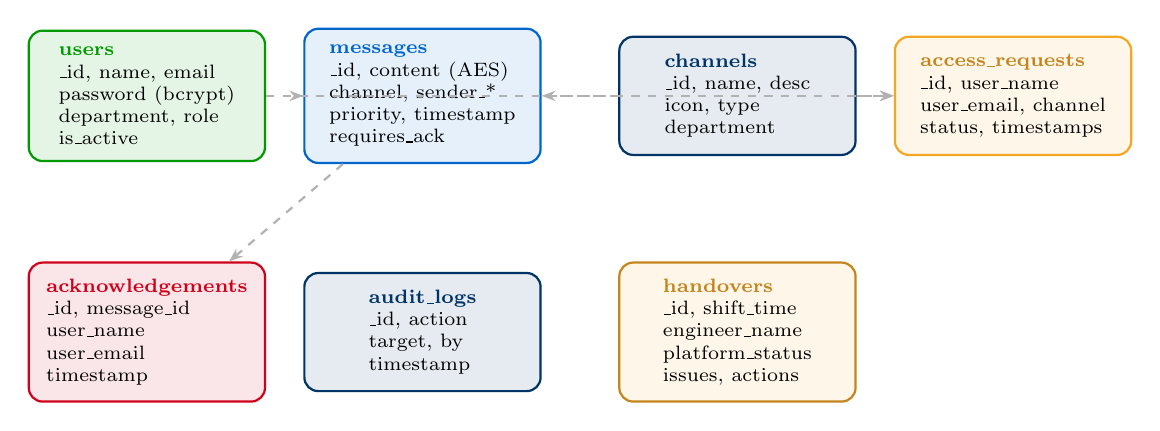
\begin{tikzpicture}[
  coll/.style={rectangle,rounded corners=5pt,minimum width=3.0cm,
               minimum height=1.5cm,align=flush left,inner sep=6pt,
               draw,thick,font=\scriptsize},
  arrow/.style={-{Stealth[length=5pt]},gray!60,dashed,thick}
]
  \node[coll,fill=BPGreen!10,draw=BPGreen] (users) at (-5,1.5) {
    \textcolor{BPGreen}{\textbf{users}}\\
    \_id, name, email\\
    password (bcrypt)\\
    department, role\\
    is\_active
  };
  \node[coll,fill=AccentBlue!10,draw=AccentBlue] (msgs) at (-1.5,1.5) {
    \textcolor{AccentBlue}{\textbf{messages}}\\
    \_id, content (AES)\\
    channel, sender\_*\\
    priority, timestamp\\
    requires\_ack
  };
  \node[coll,fill=BPDark!10,draw=BPDark] (chan) at (2.5,1.5) {
    \textcolor{BPDark}{\textbf{channels}}\\
    \_id, name, desc\\
    icon, type\\
    department
  };
  \node[coll,fill=AccentGold!10,draw=AccentGold] (access) at (6,1.5) {
    \textcolor{AccentGold!80!black}{\textbf{access\_requests}}\\
    \_id, user\_name\\
    user\_email, channel\\
    status, timestamps
  };
  \node[coll,fill=AccentRed!10,draw=AccentRed] (ack) at (-5,-1.5) {
    \textcolor{AccentRed}{\textbf{acknowledgements}}\\
    \_id, message\_id\\
    user\_name\\
    user\_email\\
    timestamp
  };
  \node[coll,fill=BPDark!10,draw=BPDark] (audit) at (-1.5,-1.5) {
    \textcolor{BPDark}{\textbf{audit\_logs}}\\
    \_id, action\\
    target, by\\
    timestamp
  };
  \node[coll,fill=AccentGold!10,draw=AccentGold!80!black] (hand) at (2.5,-1.5) {
    \textcolor{AccentGold!80!black}{\textbf{handovers}}\\
    \_id, shift\_time\\
    engineer\_name\\
    platform\_status\\
    issues, actions
  };
  \draw[arrow] (users)--(msgs);
  \draw[arrow] (msgs)--(ack);
  \draw[arrow] (chan)--(msgs);
  \draw[arrow] (users)--(access);
  \draw[arrow] (chan)--(access);
\end{tikzpicture}
\end{frame}

% ============================================================
\section{API \& WebSockets}
% ============================================================

\begin{frame}{REST API Endpoints}
\centering\small
\begin{tabular}{@{}lllp{5.5cm}@{}}
  \toprule
  \textbf{Method} & \textbf{Endpoint} & \textbf{Auth} & \textbf{Description} \\
  \midrule
  \rowcolor{BPGreen!10}
  POST & \texttt{/auth/register}          & None  & Register new \texttt{@bp.com} user \\
  \rowcolor{BPGreen!10}
  POST & \texttt{/auth/login}             & None  & Authenticate, receive JWT \\
  GET  & \texttt{/auth/users}             & JWT   & List all active users \\
  \rowcolor{BPDark!5}
  GET  & \texttt{/channels}              & JWT   & Fetch accessible channels \\
  \rowcolor{BPDark!5}
  POST & \texttt{/channels/request}       & JWT   & Request channel access \\
  \rowcolor{AccentBlue!8}
  GET  & \texttt{/messages/\{channel\}}  & JWT   & Load message history \\
  \rowcolor{AccentBlue!8}
  POST & \texttt{/messages/upload}        & JWT   & Upload file, get token URL \\
  \rowcolor{AccentBlue!8}
  GET  & \texttt{/messages/file/\{token\}}& JWT   & Download via signed token \\
  \rowcolor{AccentGold!10}
  GET  & \texttt{/handover}              & JWT   & Retrieve handover history \\
  \rowcolor{AccentGold!10}
  POST & \texttt{/handover}              & JWT   & Create new handover record \\
  \rowcolor{AccentRed!8}
  GET  & \texttt{/admin/requests}         & Admin & View access requests \\
  \rowcolor{AccentRed!8}
  POST & \texttt{/admin/requests/\{id\}}  & Admin & Approve / deny request \\
  \rowcolor{AccentRed!8}
  POST & \texttt{/admin/users/\{id\}/toggle}& Admin & Activate / deactivate user \\
  GET  & \texttt{/admin/audit}            & Admin & Retrieve audit log \\
  \bottomrule
\end{tabular}
\end{frame}

\begin{frame}{WebSocket Events (Socket.IO)}
\begin{columns}[t]
\column{0.48\textwidth}
\small\bfseries Client $\to$ Server Events
\vspace{4pt}
\begin{tcolorbox}[colback=SlideGray,colframe=BPDark,arc=4pt,
  left=4pt,right=4pt,top=4pt,bottom=4pt]
\ttfamily\scriptsize
\begin{tabular}{@{}p{0.40\textwidth}p{0.52\textwidth}@{}}
  \textcolor{AccentBlue}{connect}       & JWT in query param \\[2pt]
  \textcolor{AccentBlue}{join\_channel} & Subscribe to channel \\[2pt]
  \textcolor{AccentBlue}{send\_message} & Encrypted msg + channel \\[2pt]
  \textcolor{AccentBlue}{typing}        & Typing indicator \\[2pt]
  \textcolor{AccentBlue}{upload\_file}  & Binary file data \\[2pt]
  \textcolor{AccentBlue}{acknowledge}   & Msg acknowledgment \\[2pt]
  \textcolor{AccentBlue}{emergency}     & Emergency broadcast \\[2pt]
  \textcolor{AccentBlue}{disconnect}    & Cleanup + user list \\
\end{tabular}
\end{tcolorbox}

\column{0.48\textwidth}
\small\bfseries Server $\to$ Client Events
\vspace{4pt}
\begin{tcolorbox}[colback=SlideGray,colframe=BPGreen,arc=4pt,
  left=4pt,right=4pt,top=4pt,bottom=4pt]
\ttfamily\scriptsize
\begin{tabular}{@{}p{0.45\textwidth}p{0.47\textwidth}@{}}
  \textcolor{BPGreen}{message}         & New message to room \\[2pt]
  \textcolor{BPGreen}{user\_joined}    & Notify room of join \\[2pt]
  \textcolor{BPGreen}{user\_left}      & Notify room of leave \\[2pt]
  \textcolor{BPGreen}{online\_users}   & Updated presence list \\[2pt]
  \textcolor{BPGreen}{typing}          & Typing broadcast \\[2pt]
  \textcolor{BPGreen}{file\_uploaded}  & File URL + metadata \\[2pt]
  \textcolor{BPGreen}{ack\_update}     & Acknowledgment update \\[2pt]
  \textcolor{BPGreen}{emergency\_alert}& Full-screen broadcast \\
\end{tabular}
\end{tcolorbox}
\end{columns}

\vspace{6pt}
\begin{tcolorbox}[colback=BPDark!5,colframe=BPDark,arc=4pt,
  left=6pt,right=6pt,top=3pt,bottom=3pt]
\scriptsize\centering
\textbf{Connection Security:} Every WebSocket connection validates the JWT at the \texttt{connect} handler via \texttt{auth\_middleware}. Invalid or expired tokens are rejected before any room subscription.
\end{tcolorbox}
\end{frame}

% ============================================================
\section{Summary \& Roadmap}
% ============================================================

\begin{frame}{Feature Summary}
\begin{columns}[t]
\column{0.48\textwidth}
\small\bfseries Implemented Features
\vspace{4pt}

\begin{tcolorbox}[colback=BPGreen!8,colframe=BPGreen,arc=5pt,
  left=4pt,right=4pt,top=4pt,bottom=4pt]
\small
\begin{itemize}\setlength\itemsep{4pt}
  \item[\faCheckCircle] AES-256 end-to-end encryption
  \item[\faCheckCircle] JWT authentication + RBAC
  \item[\faCheckCircle] Real-time WebSocket messaging
  \item[\faCheckCircle] 7 channels + DMs
  \item[\faCheckCircle] Message priority levels + ACKs
  \item[\faCheckCircle] Emergency broadcast system
  \item[\faCheckCircle] Secure file sharing (20~MB, tokens)
  \item[\faCheckCircle] Digital shift handover
  \item[\faCheckCircle] Admin panel (3 tabs)
  \item[\faCheckCircle] Audit logging
  \item[\faCheckCircle] Trilingual content filtering (EN/AZ/RU)
  \item[\faCheckCircle] Online user presence tracking
  \item[\faCheckCircle] Channel access request workflow
\end{itemize}
\end{tcolorbox}

\column{0.48\textwidth}
\small\bfseries Potential Future Roadmap
\vspace{4pt}

\begin{tcolorbox}[colback=SlideGray,colframe=AccentBlue,arc=5pt,
  left=4pt,right=4pt,top=4pt,bottom=4pt]
\small
\begin{itemize}\setlength\itemsep{4pt}
  \item[\faClock] Message retention policies \& archiving
  \item[\faClock] Multi-factor authentication (TOTP)
  \item[\faClock] Mobile application (React Native)
  \item[\faClock] Push notifications (web + mobile)
  \item[\faClock] Video/voice calls (WebRTC)
  \item[\faClock] Message search \& full-text index
  \item[\faClock] True E2EE for direct messages
  \item[\faClock] SSO / Active Directory integration
  \item[\faClock] Kubernetes deployment + CI/CD
  \item[\faClock] SIEM integration for audit logs
  \item[\faClock] Advanced threat detection (ML)
  \item[\faClock] Offline-capable PWA
\end{itemize}
\end{tcolorbox}
\end{columns}
\end{frame}

% ── FINAL SLIDE ──────────────────────────────────────────────
{
\setbeamertemplate{footline}{}
\begin{frame}[plain]

\begin{tikzpicture}[remember picture,overlay]
  \fill[BPDark] (current page.south west) rectangle (current page.north east);
  \fill[BPGreen,opacity=0.12]
    ([xshift=-1cm,yshift=1cm]current page.north east) circle (7cm);
  \fill[AccentGold,opacity=0.08]
    ([xshift=2cm,yshift=-1cm]current page.south west) circle (5cm);
  \fill[BPGreen] ([xshift=0cm]current page.south west)
    rectangle ([xshift=0.6cm]current page.north west);
  % Icon
  \node[text=BPGreen,font=\fontsize{52}{52}]
    at ([xshift=0cm,yshift=1.2cm]current page.center) {\faShield};
  % Title
  \node[text=white,font=\fontsize{28}{30}\bfseries]
    at ([xshift=0cm,yshift=-0.4cm]current page.center) {Thank You};
  % Tagline
  \node[text=BPGreen!80,font=\large\bfseries]
    at ([xshift=0cm,yshift=-1.2cm]current page.center)
    {SecureDesk --- Securing Every Conversation};
  \node[text=white!60,font=\normalsize]
    at ([xshift=0cm,yshift=-1.9cm]current page.center)
    {BP Azerbaijan Enterprise Communication Platform};
  % Stats bar
  \fill[BPDark!80] ([yshift=1.5cm]current page.south west)
    rectangle ([yshift=2.5cm]current page.south east);
  \node[text=BPGreen!80,font=\bfseries\small]
    at ([xshift=2.5cm,yshift=2.0cm]current page.south) {AES-256};
  \node[text=white!50,font=\tiny]
    at ([xshift=2.5cm,yshift=1.65cm]current page.south) {Encryption};
  \node[text=BPGreen!80,font=\bfseries\small]
    at ([xshift=6cm,yshift=2.0cm]current page.south) {7+};
  \node[text=white!50,font=\tiny]
    at ([xshift=6cm,yshift=1.65cm]current page.south) {Channels};
  \node[text=BPGreen!80,font=\bfseries\small]
    at ([xshift=9.5cm,yshift=2.0cm]current page.south) {3 Roles};
  \node[text=white!50,font=\tiny]
    at ([xshift=9.5cm,yshift=1.65cm]current page.south) {RBAC};
  \node[text=BPGreen!80,font=\bfseries\small]
    at ([xshift=13cm,yshift=2.0cm]current page.south) {47+ Words};
  \node[text=white!50,font=\tiny]
    at ([xshift=13cm,yshift=1.65cm]current page.south) {AZ Filter};
  \node[text=white!30,font=\scriptsize]
    at ([xshift=0cm,yshift=0.4cm]current page.south) {May 2026};
\end{tikzpicture}
\end{frame}
}

\end{document}
